\chapter{Tuning Other Parameters}
\label{ch:parameter_tuning}

%\section{Methodology}
%
%Each parameter examined in this chapter is studied using the same four-step procedure. First, a single parameter is chosen as the subject under test, with all other parameters held at their existing defaults. Second, a Gaussian-process-based search (via Optuna) is run to find the empirically best value of that parameter for a set of common, representative transform configurations, spanning a range of problem sizes, thread counts, precisions, tolerances, and dimensionalities. Third, \texttt{perf} is used to explore how the transform's performance characteristics -- cache behaviour, DRAM traffic, branch misses, and per-function cycle share -- change between the legacy baseline and the empirically found optimum, in order to understand \emph{why} the optimum performs better rather than simply that it does. Fourth, these findings are used to develop an improved heuristic for choosing the parameter automatically, in place of the fixed default FINUFFT currently ships with.

%\section{Overview}

\section{Parameters Under Consideration}

Beyond $\sigma$, which was treated in Chapter~\ref{ch:sigma_selection}, parameters analyzed in this chapter are: the maximum subproblem size, bin size. 

FINUFFT algorithm projects non uniform points onto uniform grid. To project points in efficiently, they are first sorted into bins and then processed in batches. This chapter will analyze how both parameters under Consideration affect throughout during these stages.

\subsection{Processing of subproblem}
Processing a single subproblem during \texttt{execute} consists of three steps. \emph{Gathering} loads the coordinates and strengths of that subproblem's assigned points into a local buffer and allocates the local subgrid they will be spread onto. \emph{Spreading} then accumulates each point's contribution into that local subgrid, applying the spreading kernel over the $w^d$ neighbourhood of cells around each point. \emph{Adding} (\texttt{add\_wrapped\_subgrid}) finally writes the finished local subgrid back into the shared global fine grid.

\section{Subgrid size}
\label{sec:subgrid_size}

Subgrid size influences performance during the addition step. A subgrid is a cuboid that tightly wraps all the points assigned to its subproblem, padded by the kernel width. Subproblems themselves are picked from a partially bin-sorted array of points: rather than fully sorting all points by position, the points are only sorted into coarse bins, and each subproblem is then formed by taking a contiguous run of $S_{\max}$ points from this partially-sorted array. Because the points are randomly distributed, the subgrids of different subproblems sometimes overlap, so the sum of all subgrid areas exceeds the global area. Figure~\ref{fig:subgrid_overlap} shows how the first 20 such cuboids are written into the global grid, and how much they overlap one another along both axes.

That overlap makes itself felt twice. The first cost is direct: each cell written carries a constant store cost, so the excess area is simply extra stores. The second is indirect, since every addition to the shared grid must be synchronized, for which FINUFFT provides two options: a critical section or an atomic compare-and-swap. With a critical section, the step's performance depends only on the number of threads and subproblems. With atomic stores it depends instead on how much the subgrids overlap. There is no hardware instruction for atomic addition of floats or doubles, so OpenMP's implementation of \texttt{\#pragma omp atomic} falls back to a compare-and-swap: the old value is first loaded from the grid, then a new value is stored via a CAS that checks whether the old value is still present; a subsequent branch checks whether the CAS succeeded, and on failure the operation is retried. This gives the accumulation step the lock-free property, per the definition in~\cite[Sec.~3.7, p.~60]{herlihyshavit2012}, and makes the overlapping area set the expected number of retries. The two options therefore call for different targets: minimizing the number of subgrids with a critical section, and minimizing the overlap between them with compare-and-swap.

\subsection{Estimating average subgrid size}

Average subgrid size, given uniform distribution of points can be estimated before transform based on maximum subproblem size, bin size and density. 1d subgrid size formula is the simplest to derive. Write $\tilde{N}$ for the number of cells of the fine grid, $\rho = M/\tilde{N}$ for the average number of points per cell, $b$ for the bin size in cells, and $w$ for the kernel width. Bin sorting places on average $\rho b$ points in each bin and orders the array by bin, but leaves the points within a bin in arbitrary order, so a subproblem built from a contiguous run of $S_{\max}$ points may draw them from anywhere inside the bins that run touches. Its bounding interval is therefore the union of those bins rather than the span of the points themselves. The run consumes $S_{\max} / (\rho b)$ bins worth of points and starts at an arbitrary offset inside the first of them, so it touches
\begin{equation}
    n_b = \frac{S_{\max}}{\rho b} + 1
    \label{eq:subgrid_bins}
\end{equation}
bins on average, covering $n_b b$ cells. FINUFFT then pads that interval by half a kernel width on each side, so that spreading needs no bounds checking, which adds a further $w$ cells. The average subgrid size in one dimension is thus
\begin{equation}
    L_1 = n_b b + w = \frac{S_{\max}}{\rho} + b + w.
    \label{eq:subgrid_1d}
\end{equation}
The three terms separate the three contributions: $S_{\max}/\rho$ is the extent the points genuinely occupy, $b$ is the slack introduced by sorting only into bins rather than fully, and $w$ is the kernel padding. 

In two dimensions the bins are visited $x$ fastest, so a contiguous run of points fills entire rows of bins along $x$ before advancing in $y$. A bin-row is $b_y$ cells tall, so a strip of it one cell wide holds $\rho b_y$ points and a subproblem reaches
\begin{equation}
    x_{\mathrm{ext}} = \frac{S_{\max}}{\rho\, b_y}, \qquad
    r = \frac{x_{\mathrm{ext}}}{N_x}, \qquad
    f = \min(1, r)
    \label{eq:subgrid_xext}
\end{equation}
cells along $x$ while it stays inside one row, where $r$ expresses that reach as a fraction of a bin-row and $f$ is the probability that the run does not fit inside a single row. Which of two shapes the subgrid takes depends on where the run happens to start. If it lies entirely within one row like on Figure~\ref{fig:subgrid_cuboid_regular} it is a compact box, $x_{\mathrm{ext}} + b_x$ cells wide and $b_y$ tall. If instead it straddles a row boundary linke on Figure~\ref{fig:subgrid_cuboid_wrapping} it consists of a suffix of one row and a prefix of the next; those two pieces sit at opposite ends of the $x$ axis, so their common bounding box spans the full width of the grid and two rows in height, however few points the run holds. Figure~\ref{fig:subgrid_overlap} shows locations and dimensions of first 20 subgrids from a real transform: the compact subgrids tile each bin-row along $x$, while the straddling ones reach from edge to edge and are two rows tall. Averaging the two cases over the starting offset, and padding every extent by the kernel width, gives the mean subgrid area
\begin{equation}
    A_2 = (1 - f)\,(x_{\mathrm{ext}} + b_x + w)(b_y + w)
        \;+\; f\,(N_x + w)\bigl((\max(1, r) + 1)\, b_y + w\bigr).
    \label{eq:subgrid_2d}
\end{equation}
The two clamps play opposite roles and cannot be merged. In the first, $f = \min(1, r)$ is a probability, and it saturates at one because a run longer than a row always spans the full width. In the second, $\max(1, r)$ is a row count, and it is floored at one because a straddling run covers two rows however short it is; for $r \geq 1$ the first term vanishes and the expression reduces to $(N_1 + w)\bigl((r+1) b_y + w\bigr)$, the run starting at an arbitrary offset and therefore touching $r + 1$ rows on average.

In three dimensions the same construction applies once more, because the bins are visited $y$ next and $z$ slowest. A run now fills entire rows of bins along $x$ before advancing in $y$, and entire slabs of bins, meaning all bins sharing one $z$ index, before advancing in $z$. The reach along $x$ inside a single row becomes $x_{\mathrm{ext}} = S_{\max} / (\rho\, b_y b_z)$, and alongside $r$ and $f$ a second pair is needed for the slabs,
\begin{equation}
    q = \frac{S_{\max}}{\rho\, N_x N_y b_z} = r\,\frac{b_y}{N_y}, \qquad
    g = \min(1, q),
    \label{eq:subgrid_slab}
\end{equation}
where $q$ is the fraction of a slab a subproblem consumes and $g$ the probability that it crosses a slab boundary. Every subproblem then falls into exactly one of three cases, and since $q \leq r$ always, the probabilities partition cleanly: with probability $1 - f$ the run stays inside one row and its subgrid is compact; with probability $f - g$ it crosses a row boundary but not a slab boundary, so it spans the full width in $x$ while remaining a few rows tall; and with probability $g$ it crosses a slab boundary, whereupon the suffix and prefix it holds lie at opposite corners of an $x$--$y$ plane and the subgrid spans that plane entirely. Averaging over the three gives
\begin{equation}
    \begin{split}
    A_3 = {}& (1 - f)\,(x_{\mathrm{ext}} + b_x + w)(b_y + w)(b_z + w) \\
          &+ (f - g)\,(N_x + w)\bigl((\max(1, r) + 1)\, b_y + w\bigr)(b_z + w) \\
          &+ g\,(N_x + w)(N_y + w)\bigl((\max(1, q) + 1)\, b_z + w\bigr),
    \end{split}
    \label{eq:subgrid_3d}
\end{equation}
which reduces to \eqref{eq:subgrid_2d} in two dimensions, where there are no slabs to cross and $g = 0$.

The slab-crossing subgrids are rare but decisive, and their number is fixed by the geometry rather than by the tuning parameter: there are $N_z / b_z$ slabs, so however small $S_{\max}$ is made, that many subproblems still span a full $x$--$y$ plane each. In the measurements below this is $53$ subgrids at every $S_{\max}$, out of populations ranging from $40$ to $20{,}000$. Equation~\eqref{eq:subgrid_3d} reproduces the logged three-dimensional subgrid sizes to within $0.3\%$ across a five-hundredfold range of $S_{\max}$, covering all three regimes.

Figure~\ref{tab:subgrid_pred} compares the three predictions against subgrid sizes logged directly from the spreader, at unit density and with $b_x = 16$, $b_y = b_z = 4$ and $w = 7$. Each row averages every subgrid built during one transform, from $40$ subgrids at the largest subproblem size up to $20{,}000$ at the smallest. All three agree to within $1\%$, and the residual is largest at small $S_{\max}$, where the discrete number of bins a run touches is least well described by its average.

\begin{figure}[h]
    \centering
    \scriptsize
    \setlength{\tabcolsep}{2.5pt}
    \begin{subfigure}[t]{0.32\textwidth}
        \centering
        \begin{tabular}{rrrr}
            \hline
            $S_{\max}$ & Pred. & Meas. & Err. \\
            \hline
            0.5k   & 523    & 518    & $+0.91\%$ \\
            1k     & 1023   & 1018   & $+0.47\%$ \\
            2.5k   & 2523   & 2518   & $+0.19\%$ \\
            5k     & 5023   & 5018   & $+0.10\%$ \\
            10k    & 10023  & 10018  & $+0.05\%$ \\
            25k    & 25023  & 25018  & $+0.02\%$ \\
            50k    & 50023  & 50018  & $+0.01\%$ \\
            100k   & 100023 & 100018 & $+0.00\%$ \\
            \hline
        \end{tabular}
        \caption{1D, $N = 10^7$.}
        \label{tab:subgrid_1d}
    \end{subfigure}
    \hfill
    \begin{subfigure}[t]{0.32\textwidth}
        \centering
        \begin{tabular}{rrrr}
            \hline
            $S_{\max}$ & Pred. & Meas. & Err. \\
            \hline
            0.5k   & 3442   & 3427   & $+0.46\%$ \\
            1k     & 6523   & 6509   & $+0.21\%$ \\
            2.5k   & 15112  & 15100  & $+0.08\%$ \\
            5k     & 27255  & 27248  & $+0.03\%$ \\
            10k    & 43390  & 43374  & $+0.04\%$ \\
            25k    & 59910  & 59897  & $+0.02\%$ \\
            50k    & 84961  & 84924  & $+0.04\%$ \\
            100k   & 135063 & 134979 & $+0.06\%$ \\
            \hline
        \end{tabular}
        \caption{2D, $N_x = N_y = 3162$.}
        \label{tab:subgrid_2d}
    \end{subfigure}
    \hfill
    \begin{subfigure}[t]{0.32\textwidth}
        \centering
        \begin{tabular}{rrrr}
            \hline
            $S_{\max}$ & Pred. & Meas. & Err. \\
            \hline
            0.5k   & 12776  & 12782  & $-0.05\%$ \\
            1k     & 21683  & 21712  & $-0.14\%$ \\
            2.5k   & 41890  & 41870  & $+0.05\%$ \\
            5k     & 59739  & 59639  & $+0.17\%$ \\
            10k    & 91857  & 91672  & $+0.20\%$ \\
            25k    & 183661 & 183159 & $+0.27\%$ \\
            50k    & 321500 & 320590 & $+0.28\%$ \\
            100k   & 540295 & 539013 & $+0.24\%$ \\
            250k   & 807026 & 805710 & $+0.16\%$ \\
            \hline
        \end{tabular}
        \caption{3D, $N_x = N_y = N_z = 215$.}
        \label{tab:subgrid_3d}
    \end{subfigure}
    \caption{Predicted against measured subgrid size, from \eqref{eq:subgrid_1d}, \eqref{eq:subgrid_2d} and \eqref{eq:subgrid_3d}, at unit density with $M = 10^7$.}
    \label{tab:subgrid_pred}
\end{figure}

%How much overlap there is to minimize depends on the dimension. In one dimension a subgrid is an interval, so two subgrids can only overlap in the padding they share at a common endpoint. In two and three dimensions the subgrids are rectangles and cuboids that overlap along entire faces, and the domain boundary adds a further source of overlap on top of that. Figure~\ref{fig:subgrid_cuboid_regular} shows the regular case: since the run of points making up the subproblem is spatially localised, its bounding cuboid is a single compact rectangle. Because the fine grid is periodic, however, a subproblem whose points straddle the domain boundary produces a cuboid that must wrap around to the opposite edge, as in Figure~\ref{fig:subgrid_cuboid_wrapping}. It is then effectively split across both edges of the domain and spans almost the full extent of that axis, so it overlaps far more of the other subgrids than its point count alone would suggest.

%These two parameters are not independent. The bin size determines how spatially spread a
%contiguous run of bin-sorted points is, and $S_{\max}$ determines how many such points a
%subproblem holds; together they fix the subgrid that must be zeroed, spread into, and
%accumulated back. Tuning either one against a fixed value of the other therefore risks
%optimising along a single axis of a joint optimum. 

%To establish how much is available
%from the pair, a Gaussian-process search  was run over $S_{\max}$ and the
%bin sizes \emph{jointly} -- a two- to four-dimensional space depending on
%dimensionality -- for $1\,$GiB type-1 transforms at unit density, in both precisions and
%both single-threaded and fully parallel, giving twelve configurations.
%
%Table~\ref{tab:joint_search_summary} reports the outcome. Each searched optimum and the
%corresponding FINUFFT default were then re-run on five independently generated point
%sets (the same five for both, so that the point set cancels in the ratio); the quoted
%figure is the mean speedup over those five pairings and its standard deviation.
%
%\begin{table}[h]
%    \centering
%    \small
%    \begin{tabular}{|l|l|r|r|l|r|l|}
%        \hline
%        \textbf{Dim} & \textbf{Prec} & \textbf{Threads} & \textbf{Best $S_{\max}$}
%            & \textbf{Best bins} & \textbf{Default $S_{\max}$} & \textbf{Speedup} \\
%        \hline
%        1 & double & 1  & 3{,}231     & $(245)$        & 10{,}000  & $1.011 \pm 0.004$ \\
%        \hline
%        1 & double & 64 & 836         & $(72)$         & 10{,}000  & $1.013 \pm 0.053$ \\
%        \hline
%        1 & single & 1  & 1{,}075     & $(29)$         & 10{,}000  & $1.010 \pm 0.008$ \\
%        \hline
%        1 & single & 64 & 15{,}420    & $(336)$        & 10{,}000  & $1.013 \pm 0.016$ \\
%        \hline
%        2 & double & 1  & 312{,}474   & $(4,13)$       & 100{,}000 & $1.017 \pm 0.005$ \\
%        \hline
%        2 & double & 64 & 107{,}019   & $(4,2)$        & 100{,}000 & $1.033 \pm 0.051$ \\
%        \hline
%        2 & single & 1  & 509{,}791   & $(72,15)$      & 100{,}000 & $1.027 \pm 0.008$ \\
%        \hline
%        2 & single & 64 & 148{,}244   & $(18,2)$       & 100{,}000 & $0.995 \pm 0.023$ \\
%        \hline
%        3 & double & 1  & 1{,}719{,}564 & $(8,3,2)$    & 100{,}000 & $\mathbf{1.149 \pm 0.001}$ \\
%        \hline
%        3 & double & 64 & 1{,}603{,}666 & $(9,1,2)$    & 100{,}000 & $\mathbf{1.129 \pm 0.058}$ \\
%        \hline
%        3 & single & 1  & 1{,}213{,}511 & $(7,4,3)$    & 100{,}000 & $\mathbf{1.322 \pm 0.014}$ \\
%        \hline
%        3 & single & 64 & 1{,}996{,}464 & $(106,102,3)$ & 100{,}000 & $\mathbf{1.166 \pm 0.012}$ \\
%        \hline
%    \end{tabular}
%    \caption{Joint Gaussian-process search over $S_{\max}$ and bin sizes, for $1\,$GiB type-1 transforms at unit density. Speedup is against the FINUFFT default for that dimensionality ($S_{\max}=10^4$ in 1D, $10^5$ in 2D and 3D; bin sizes $16$, $4$, $4$), as the mean over five paired point sets $\pm$ one standard deviation.}
%    \label{tab:joint_search_summary}
%\end{table}

%The result is clear-cut: \textbf{only three-dimensional transforms admit a significant
%improvement from these two parameters.} All four 3D configurations gain between $13\%$
%and $32\%$, and the single-threaded double-precision case is reproducible to within
%$0.1\%$ across point sets. Every 1D and 2D configuration, by contrast, lies between
%$0.995$ and $1.033$ -- a margin that its own standard deviation either matches or
%exceeds, and one configuration is in fact marginally \emph{slower} than the default.
%The shipped defaults are therefore already at the optimum in one and two dimensions,
%and the remainder of this chapter concentrates on where the headroom actually is.
%
%Two features of the 3D optima explain where that headroom comes from. First, every one
%selects an $S_{\max}$ between $1.2$ and $2.0$ million, some $12$--$20\times$ the shipped
%$10^5$: in three dimensions the extra points padding each subgrid are paid on all three
%axes, so small subproblems are dominated by padding and the accumulate step suffers
%accordingly (Section~\ref{sec:cache_aware_subproblem}). Second, the standard deviations
%are an order of magnitude larger at $64$ threads than at one ($0.012$--$0.058$ against
%$0.001$--$0.014$), across every dimensionality -- the run-to-run spread is set by
%thread-scheduling and accumulation contention rather than by the parameters under test,
%which is why the small 1D and 2D margins cannot be resolved at high thread counts.

\begin{figure}[h]
    \centering
    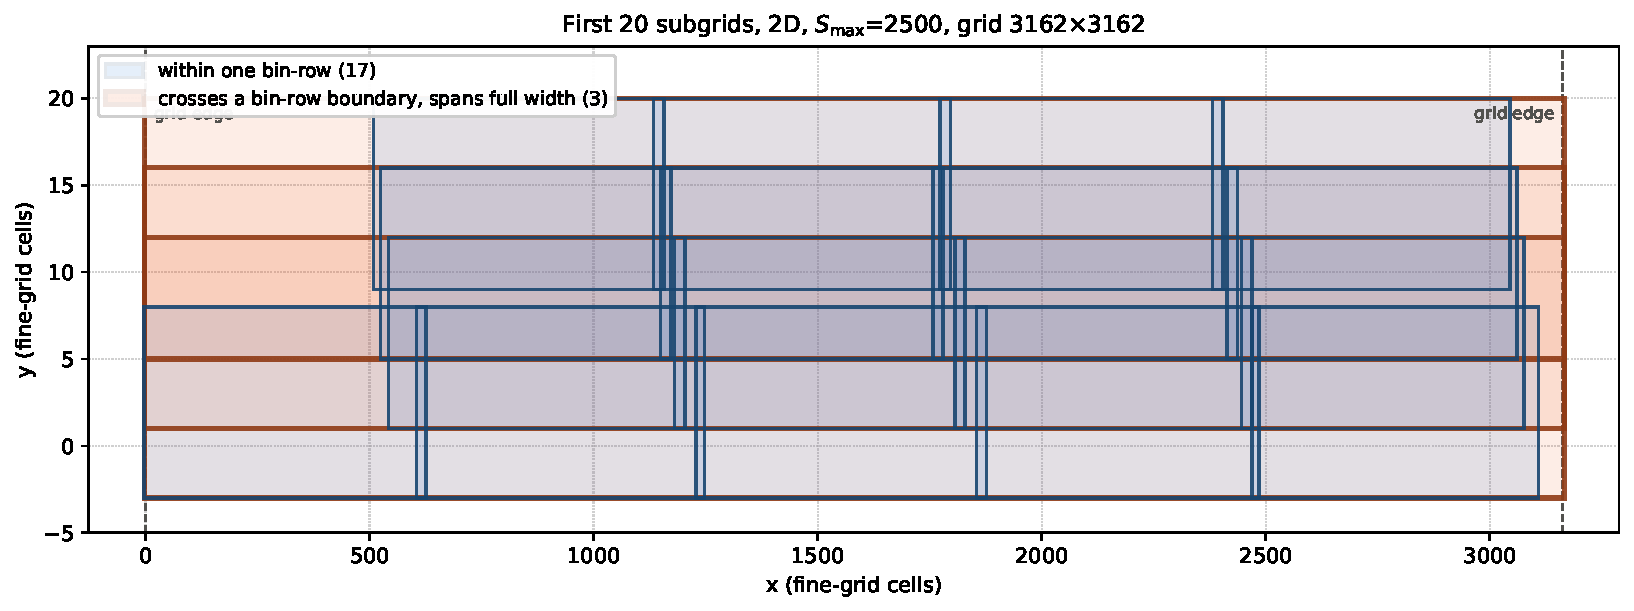
\includegraphics[width=\textwidth]{figures/subgrid_layout/subgrid_layout.pdf}
    \caption{Bounding boxes of the first 20 subgrids at $S_{\max}=2500$, coloured by whether the subproblem crosses a bin-row boundary.}
    \label{fig:subgrid_overlap}
\end{figure}

\begin{figure}[h]
    \centering
    \begin{subfigure}[b]{0.48\textwidth}
        \centering
        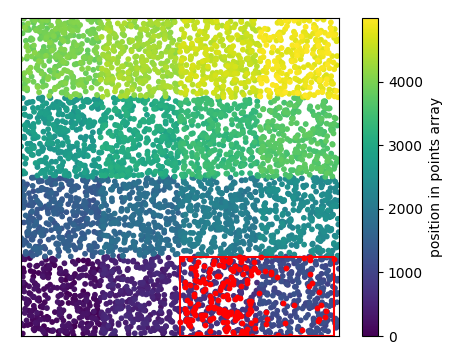
\includegraphics[width=\textwidth]{figures/bin_size/subgrid_cuboid_regular.png}
        \caption{Compact subgrid}
        \label{fig:subgrid_cuboid_regular}
    \end{subfigure}
    \hfill
    \begin{subfigure}[b]{0.48\textwidth}
        \centering
        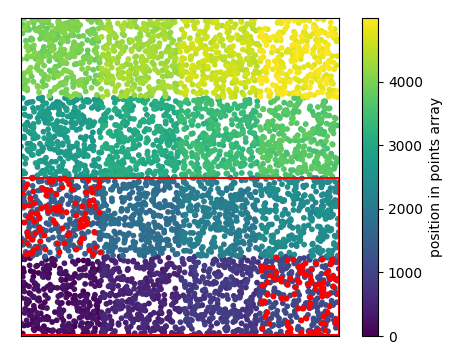
\includegraphics[width=\textwidth]{figures/bin_size/subgrid_cuboid_wrapping.png}
        \caption{Wrapping subgrid}
        \label{fig:subgrid_cuboid_wrapping}
    \end{subfigure}
    \caption{Points of one subproblem (red) among all nonuniform points, coloured by position in the sorted array.}
    \label{fig:subgrid_cuboid_examples}
\end{figure}

Both the maximum subproblem size and the bin size therefore act on the same quantity, but not in the same way. $S_{\max}$ enters only through $x_{\mathrm{ext}}$, and does so linearly: halving it halves the reach of a subproblem along the fast axis. Of the bin dimensions only $b_x$ is linear, contributing the additive slack that comes from sorting into bins rather than sorting fully. The dimensions beyond $x$ are not. Because $b_y$ sits in the denominator of $x_{\mathrm{ext}}$, it also enters $r$ and the crossing probability $f$: enlarging it shortens the reach along $x$ and makes a boundary crossing less likely, while at the same time making every row taller and every crossing that does occur more expensive. In three dimensions $b_z$ repeats the pattern one level up, through $q$.

\section{Maximum Subproblem Size}

During the spreading phase, nonuniform points are partitioned into spatially localised subproblems so that each subproblem's contribution to the fine grid can be accumulated independently. The parameter $S_{\max}$ (exposed in the FINUFFT interface as \texttt{max\_subproblem\_size}) sets an upper bound on the number of nonuniform points assigned to any single subproblem.

A larger $S_{\max}$ reduces the total number of subproblems, thereby lowering scheduling and synchronisation overhead. However, if subproblems are too large relative to the number of available threads, work is distributed unevenly and some threads may sit idle while others finish their chunk, reducing parallel efficiency.

$S_{\max}$ determines the amount of memory dedicated to subproblem processing. During the gathering step, the algorithm loads this number of points with their coordinates into the memory buffer.
Finally, $S_{\max}$ fixes the size of the subgrid for each subproblem, through the relations derived in Section~\ref{sec:subgrid_size}: \eqref{eq:subgrid_1d} in one dimension, \eqref{eq:subgrid_2d} in two and \eqref{eq:subgrid_3d} in three. 

Figure~\ref{fig:maxsp_steps} measures the three steps separately across the range, on a 2D transform of $1$\,GiB of nonuniform points at unit density. The two costs move against each other: adding falls as fewer, larger subproblems write back less redundantly, while gathering rises. At the same time spreading step becomes slower, but not as significantly as gathering. 


The same three steps in cycles rather than wall time are shown in Figure~\ref{fig:maxsp_cycles}, and the two views disagree. Counted in cycles, adding falls by a factor of $5.5$ across the range and spreading is flat, drifting down by a quarter; only gathering grows, and it stops doing so beyond $S_{\max} \approx 10^5$. Counted in wall-clock time, all three are worse at the top of the range: spreading rises by $1.7$ and adding falls by only $2.3$ rather than $5.5$.

Cycles count work actually performed, summed over threads, so comparing the two figures separates a real slowdown from wall time inflated by idle threads. Gathering costs $1.7$ times more cycles at the top of the range than at the bottom and stops growing beyond $S_{\max} \approx 10^5$, whereas its wall-clock cost keeps rising to $3.8$ times. The difference is load imbalance: at the largest subproblem sizes there is barely one subproblem per thread, so the phase ends only when the slowest thread finishes and the others wait.

\begin{figure}[h]
    \centering
    \begin{subfigure}[b]{0.49\textwidth}
        \centering
        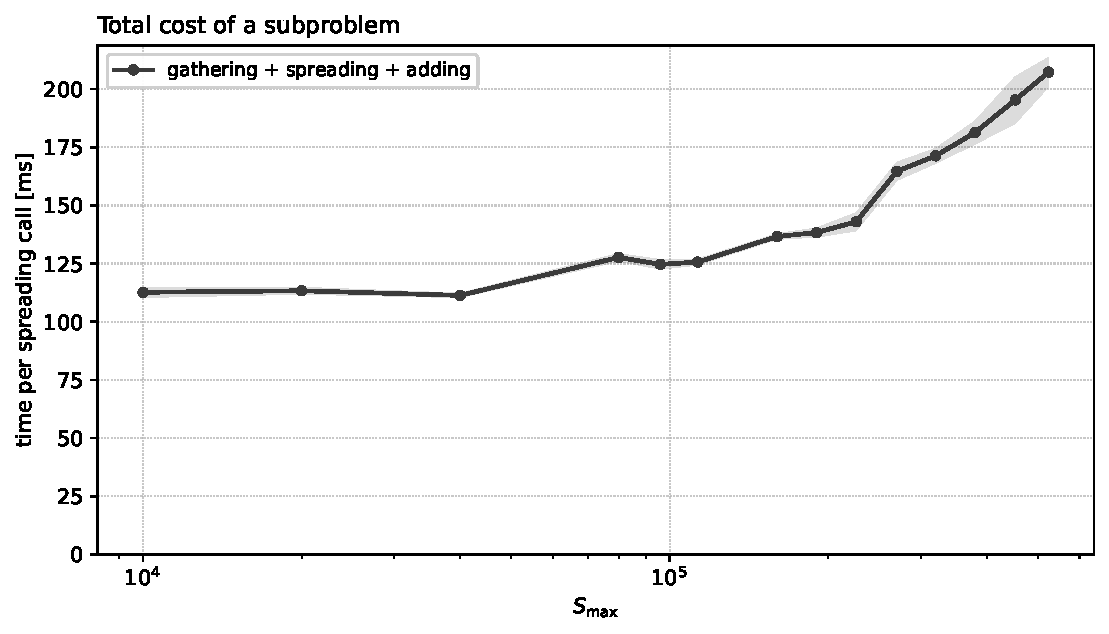
\includegraphics[width=\textwidth]{figures/maxsp_steps/maxsp_steps.pdf}
        \caption{Wall-clock time.}
        \label{fig:maxsp_steps}
    \end{subfigure}
    \hfill
    \begin{subfigure}[b]{0.49\textwidth}
        \centering
        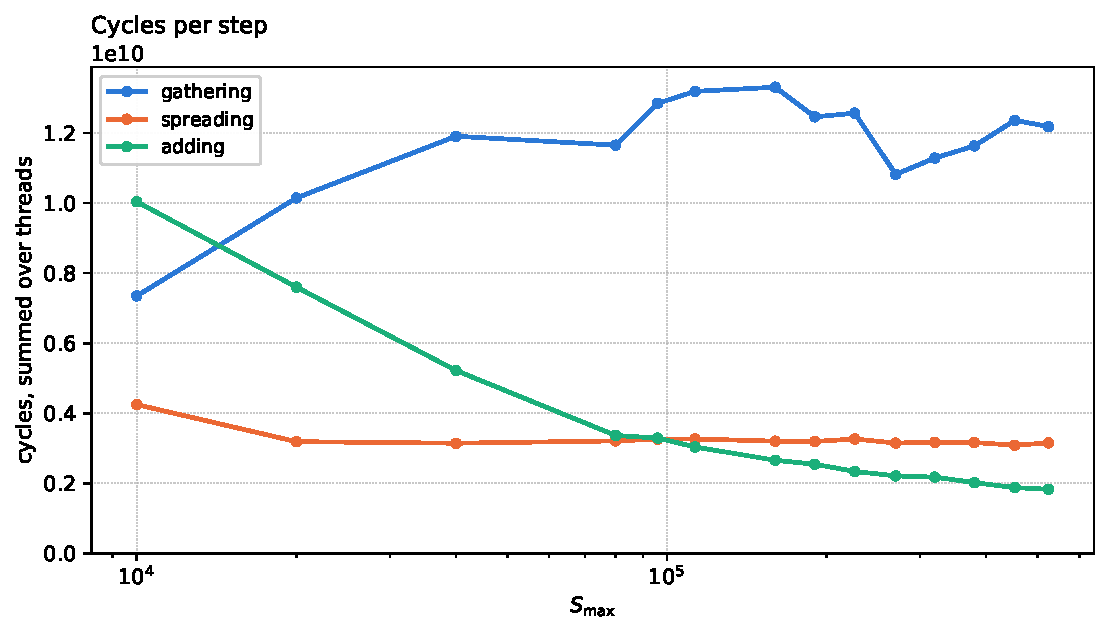
\includegraphics[width=\textwidth]{figures/maxsp_steps/maxsp_cycles.pdf}
        \caption{Cycles, summed over threads.}
        \label{fig:maxsp_cycles}
    \end{subfigure}
    \caption{Cost of gathering, spreading and adding against $S_{\max}$, measured as wall-clock time and as cycles.}
    \label{fig:maxsp_steps_pair}
\end{figure}


\subsection{Older heuristics}
The current heuristic sets $S_{\max}$ to the minimum of $10^5$ and $N/n_{\text{thr}}$ for type-2 and type-3 transforms, and to the minimum of $10^4$ and $N/n_{\text{thr}}$ for type-1 transforms. These constants are suboptimal: they introduce extra OpenMP scheduling overhead, and for transforms with very low density, the subgrid can end up very large and spill out of cache into main memory.


\subsection{Effect on gathering.}
Each thread allocates a buffers for holding a
set of point coordinates and strengths for the current subproblem. Their combined size is
\begin{equation}
  B(S_{\max}) \;=\; S_{\max}\,\cdot\,\texttt{sizeof(FLT)}\,\cdot\,(d+2),
  \label{eq:staging_buffer}
\end{equation}
with $d$ words per point for the coordinates and two for the complex strength.  While $B(S_{\max})$ fits in a thread's share of cache, the
lines written by one subproblem are still owned when the next one overwrites them, and the
stores cost nothing beyond the cache hit. Once $B(S_{\max})$ exceeds that share, every
written line, with points, must first be fetched for ownership and later written back.
CPU uses line-fill buffers that bring back cache line from lower hierarchy levels. When pool of buffers is exhausted
gathering cycles begin to stall.
Figure~\ref{fig:fb_full} shows the mechanism directly: the
\texttt{l1d\_pend\_miss.fb\_full} counter, which records the cycles a demand request was
blocked because no fill buffer was available, rises by a third across the range and
climbs fastest over the same interval in which gathering does, before flattening once
the buffer is far larger than the cache can hold. The
\texttt{cycle\_activity.stalls\_l3\_miss} counter, which records cycles stalled on a
demand load that missed the last-level cache, grows over that same interval, by a
fifth, and flattens at the same point. Both counters therefore rise and slow down gathering.

\begin{figure}[h]
    \centering
    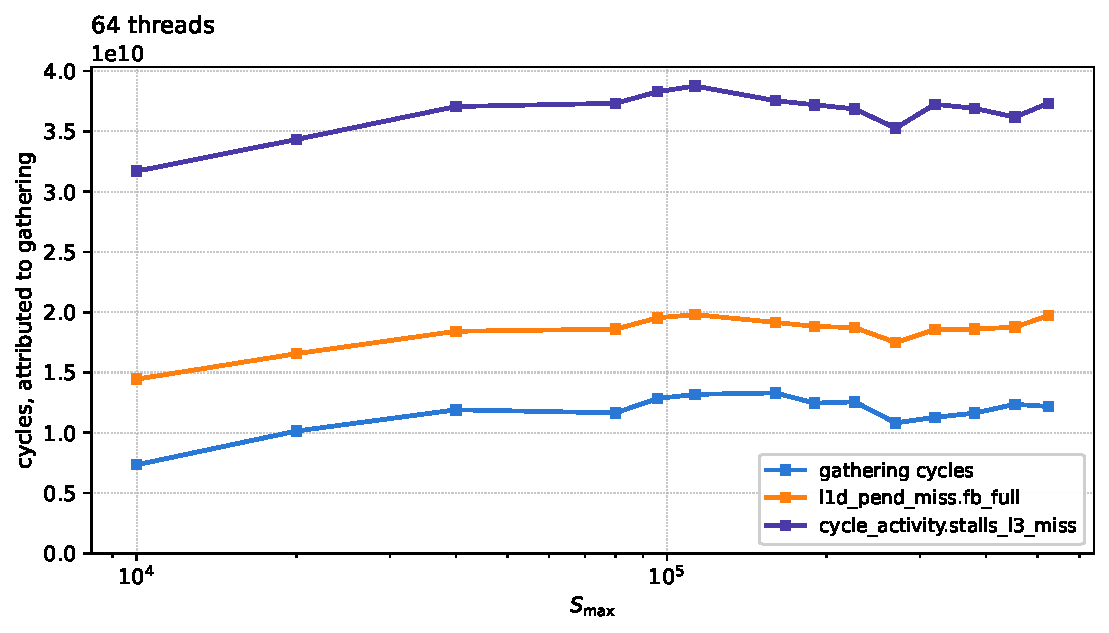
\includegraphics[width=\textwidth]{figures/maxsp_steps/maxsp_fbfull.pdf}
    \caption{Cycles consumed by gathering, the fill-buffer stalls and the L3-miss stalls attributed to it, against $S_{\max}$, on 64 threads.}
    \label{fig:fb_full}
\end{figure}
\subsection{Effect on adding.}
The adding step walks every cell of the local subgrid, so its cost is proportional to
$n_{\text{sub}} \cdot A(S_{\max})$, the total number of padded cells summed over all
subproblems. Each subgrid is padded by the kernel width $w$ in every dimension, and those
extra points are a fixed cost per subproblem rather than per point: reducing $S_{\max}$
raises the number of subproblems and therefore raises how many extra points must be
traversed, even though each individual subgrid is smaller. Adding is also the more expensive operation per cell,
since it accumulates into the shared fine grid under an atomic update.

Figure~\ref{fig:maxsp_addvol} shows the measured adding time alongside the write volume the
subgrid model predicts, $A(S_{\max}) \cdot n_{\mathrm{sub}}$. Adding time is almost perfectly
predicted by the number of cells written.

\begin{figure}[h]
    \centering
    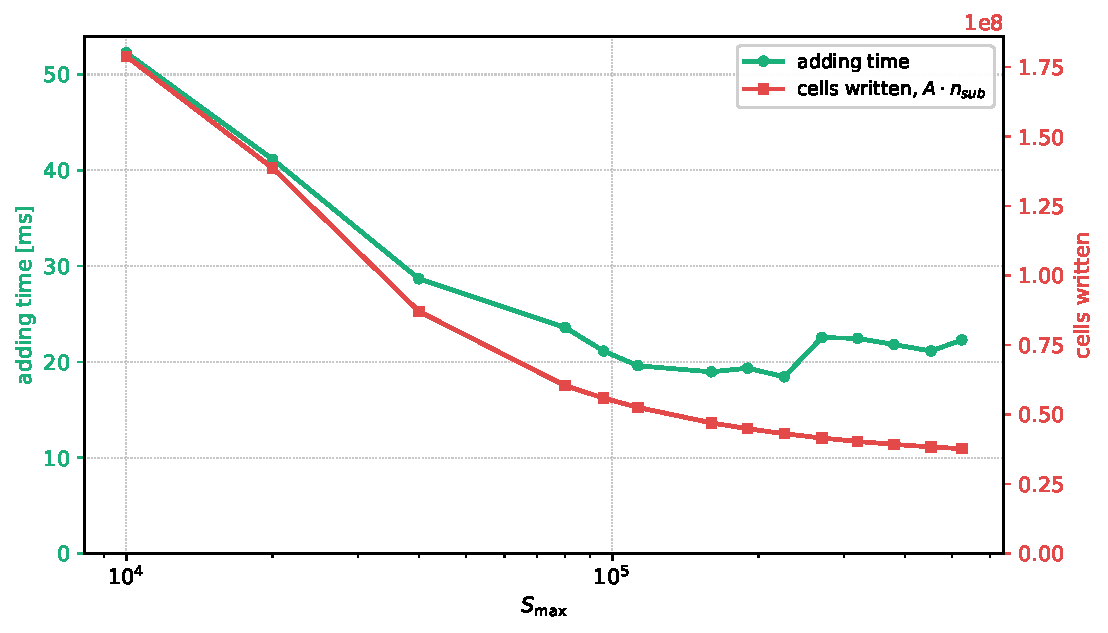
\includegraphics[width=0.8\textwidth]{figures/maxsp_steps/maxsp_addvol.pdf}
    \caption{Measured adding time and the number of cells written predicted by the subgrid model, against $S_{\max}$.}
    \label{fig:maxsp_addvol}
\end{figure}

\subsection{Relative effects of gathering and adding}


Transform density, the number of nonuniform points per grid cell, determines the balance
between gathering and adding. At high density a full buffer of points spans only a small
region of the grid, whereas at low density the opposite happens and even a small buffer
spreads across a large subgrid. Small subproblems therefore perform better when density is
high, and large subproblems when density is low. The first two panels of
Figure~\ref{fig:maxsp_density} show the two extremes: at $\rho = 0.125$ adding dominates
throughout and falls as $S_{\max}$ grows, while at $\rho = 16$ it is already small and
gathering, which rises, decides the choice. Finally, in single-threaded transforms gathering
time does not change much with $S_{\max}$, as the third panel of the same figure shows, so it
is better to use large subproblems and minimise the total number of cells written. The full
sweep, over every combination of dimension, density and thread count, is given in
Appendix~\ref{app:smax_sweep_full}.

\begin{figure}[h]
    \centering
    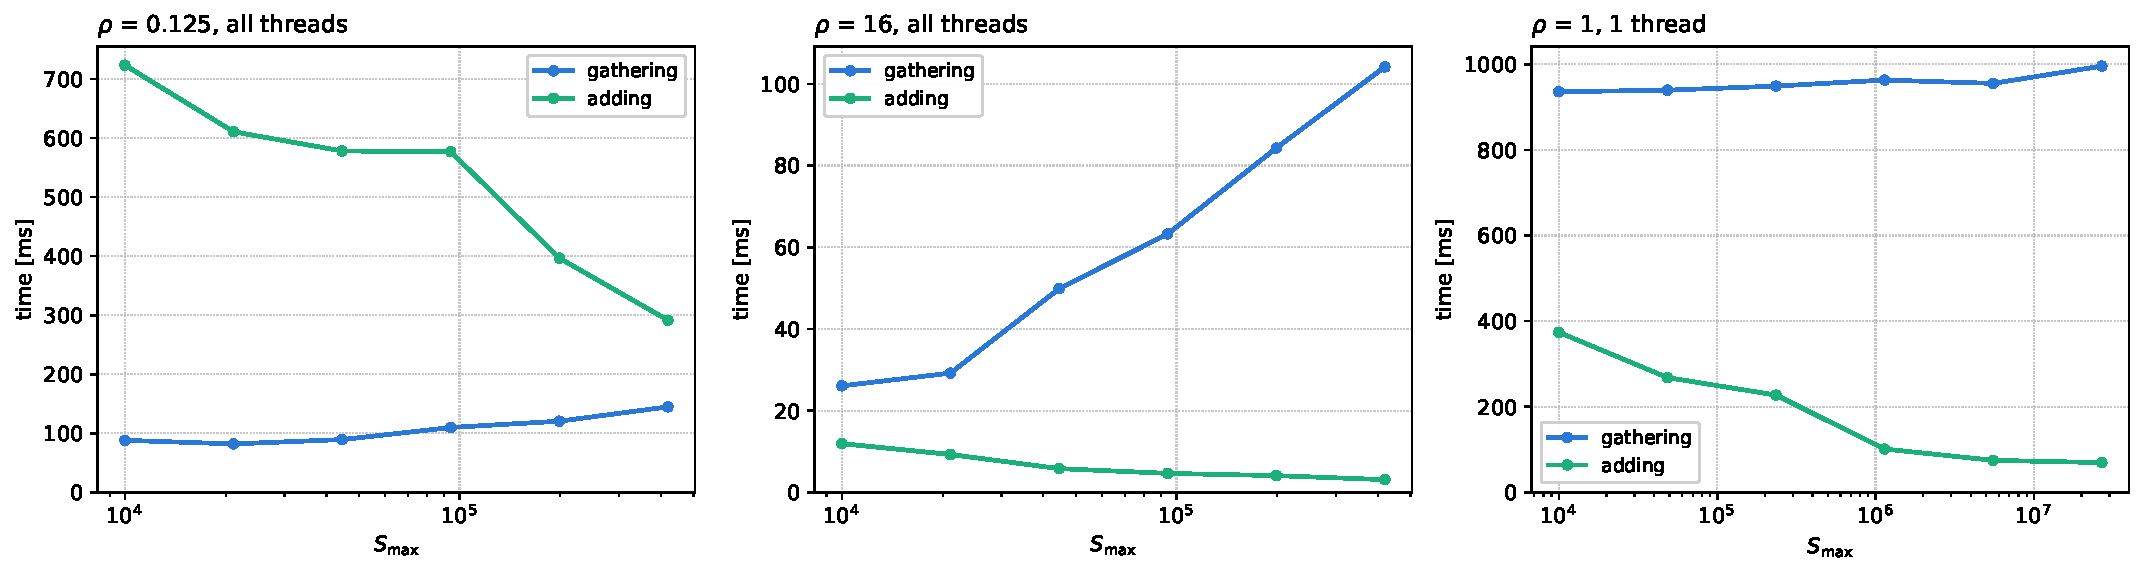
\includegraphics[width=\textwidth]{figures/maxsp_density/maxsp_density.pdf}
    \caption{Gathering and adding time against $S_{\max}$ at low and high point density, and at unit density on a single thread.}
    \label{fig:maxsp_density}
\end{figure}


\section{Binsize}

FINUFFT does not fully sort points by position before spreading. It instead relies on an \emph{incomplete} histogram sort, built from three passes: tallying how many points fall into each bin and converting those tallies into bin breakpoints; placing each point's index into its bin's slot; and reading the indices back out one bin at a time, with no ordering imposed on points sharing a bin. Because this scheme operates entirely on per-bin counters rather than comparisons between points, its running time is governed by how many bins there are, not by how many points are being sorted -- so it stays fast precisely when that counter array is small enough to remain in cache, making it the quickest available method for this coarse spatial grouping.

By default, FINUFFT sets up boxes of size 16 grid points in the fast ($x$) dimension, and, in 2D or 3D, size 4 in the slower ($y$ and $z$) dimensions. These sizes can be optimized based on the transform being run.

Bin size does not only affect this sorting step, however -- it also affects the subgrids formed downstream. A larger bin size means each bin covers a larger, coarser region of space, so a contiguous run of $S_{\max}$ points drawn from a coarser bin ordering is more spatially spread out, and the bounding cuboid needed to enclose them grows accordingly. Past a certain point, this makes the subgrid too large, which in turn slows down the adding step: since \texttt{add\_wrapped\_subgrid} must write out every subgrid cell, its cost can be quantified as the number of subproblems multiplied by the average subgrid size. Choosing the bin size is therefore a matter of balancing two opposing effects: a coarser bin size speeds up sorting but inflates subgrids and slows down adding, while a finer bin size keeps subgrids compact but makes sorting itself more expensive.

The same reasoning applies in every dimension, with one factor per axis. Write $n_i$
for the fine-grid extent along axis $i$, $\beta_i$ for the bin size, $\rho$ for the
density, $w$ for the kernel width and $b$ for the bytes per cell. Along the fastest
axis a subproblem either covers a fraction $f$ of the full extent or, when its points
fit inside a single bin, just that bin plus the kernel halo; along each slower axis it
spans however many bins its points reach into, again plus the halo. In one dimension
there is only the fast axis:
\begin{align*}
    f &= \min\!\left(1,\; \frac{S}{n_1 \rho}\right), \\
    A(S) &= \left[\, n_1 f + (1-f)\beta_1 + w \,\right] b .
\end{align*}
In two dimensions a second axis is added, measured in whole bins:
\begin{align*}
    f &= \min\!\left(1,\; \frac{S}{n_1 \beta_2 \rho}\right), \\
    \text{size}_1 &= n_1 f + (1-f)\beta_1 + w, \\
    \text{size}_2 &= \left\lceil \frac{S}{n_1 \beta_2 \rho} \right\rceil \beta_2 + w, \\
    A(S) &= \text{size}_1 \cdot \text{size}_2 \cdot b .
\end{align*}
In three dimensions the first two axes each get their own fraction, since a subproblem
may fill one of them without filling the next, and only the slowest axis is counted in
whole bins:
\begin{align*}
    f_1 &= \min\!\left(1,\; \frac{S}{n_1 \beta_2 \beta_3 \rho}\right), &
    \text{size}_1 &= n_1 f_1 + (1-f_1)\beta_1 + w, \\
    f_2 &= \min\!\left(1,\; \frac{S}{n_1 n_2 \beta_3 \rho}\right), &
    \text{size}_2 &= n_2 f_2 + (1-f_2)\beta_2 + w, \\
    &&\text{size}_3 &= \left\lceil \frac{S}{n_1 n_2 \rho} \right\rceil \beta_3 + w, \\
    &&A(S) &= \text{size}_1 \cdot \text{size}_2 \cdot \text{size}_3 \cdot b .
\end{align*}
The $\lceil\cdot\rceil$ on the slowest axis is the source of a practical pitfall: it
makes $A(S)$ a step function there, so a value of $S_{\max}$ landing just above an
integer pays for a whole extra bin row it barely uses.

\subsection{Heuristic}
To see both effects at once, the bin size was swept over the family
$\beta_1 \times \beta_2 = 16n \times 4n$ (i.e.\ scaling the default $16\times4$ by $n$)
for a 2D type-1 double-precision transform with $n_1=n_2=10{,}000$, $M=10^8$,
$\text{tol}=10^{-6}$, on 16 threads, with $S_{\max}$ left to the cache-aware heuristic
of the previous section. Cycle counts for the three phases were attributed with
\texttt{perf}: sorting is \texttt{bin\_sort\_multithread\_impl}, spreading is
\texttt{spread\_subproblem\_2d}, and adding is \texttt{add\_wrapped\_subgrid}.

\begin{table}[h]
    \centering
    \resizebox{\textwidth}{!}{%
    \begin{tabular}{|l|r|r|r|r|r|r|r|}
        \hline
        \textbf{$\beta_1\times\beta_2$} & \textbf{Bins} & \textbf{Bins/L1d}
            & \textbf{$n_{\text{sub}} \cdot A$} & \shortstack{\textbf{Sort}\\\scriptsize\texttt{bin\_sort\_multithread\_impl}} & \shortstack{\textbf{Spread}\\\scriptsize\texttt{spread\_subproblem\_2d}}
            & \shortstack{\textbf{Add}\\\scriptsize\texttt{add\_wrapped\_subgrid}} & \textbf{Throughput (M nupts/s)} \\
        \hline
        $16\times4$    & 2{,}444{,}532 & $298\times$ & $7.50\times10^8$ & 66.5 & 29.1 & 46.3 & 13.72 \\
        \hline
        $32\times8$    & 611{,}133     & $75\times$  & $5.57\times10^8$ & 64.1 & 24.2 & 14.2 & 19.44 \\
        \hline
        $48\times12$   & 271{,}962     & $33\times$  & $4.95\times10^8$ & 52.6 & 27.5 & 12.5 & 20.97 \\
        \hline
        $64\times16$   & 153{,}272     & $19\times$  & $4.66\times10^8$ & 38.2 & 24.5 & 10.7 & 20.46 \\
        \hline
        $96\times24$   & 68{,}251      & $8.3\times$ & $4.44\times10^8$ & 31.7 & 31.7 & 9.9  & 21.63 \\
        \hline
        $128\times32$  & 38{,}318      & $4.7\times$ & $4.42\times10^8$ & 25.5 & 36.0 & 11.4 & 22.49 \\
        \hline
        $192\times48$  & 17{,}226      & $2.1\times$ & $4.70\times10^8$ & 15.5 & 33.8 & 11.7 & 22.80 \\
        \hline
        $256\times64$  & 9{,}604       & $1.2\times$ & $5.39\times10^8$ & 10.1 & 34.9 & 13.8 & 23.43 \\
        \hline
        $384\times96$  & 4{,}323       & $0.5\times$ & $1.01\times10^9$ & 7.9  & 50.6 & 34.4 & 20.17 \\
        \hline
    \end{tabular}%
    }
    \caption{Bin-size sweep over $16n\times4n$ for a 2D type-1 transform ($n_1=n_2=10{,}000$, $M=10^8$, double precision, 16 threads). Cycle counts are in billions, attributed per phase by \texttt{perf}; \textbf{Bins/L1d} is the per-thread sort histogram ($4$ bytes per bin) as a multiple of the $32\,$KiB L1 data cache.}
    \label{tab:binsize_sweep_2d}
\end{table}

The sweep separates the three phases cleanly. \emph{Sorting} falls monotonically by a
factor of $8$ (66.5 to 7.9 billion cycles) as the bins coarsen, and it tracks the
\textbf{Bins/L1d} column rather than the bin size directly: the histogram is one private
$4$-byte counter per bin per thread, so sorting is a scatter whose working set is
$4\beta^{-1}$-sized, and its cost drops steeply as that working set approaches the L1
data cache, flattening once it fits. \emph{Adding} follows $n_{\text{sub}}A$, as expected
from its cost model: both reach their minimum together at $96\times24$--$128\times32$
($4.4\times10^8$ cells, $9.9$--$11.4$ billion cycles) and both climb again beyond it.
\emph{Spreading} is the phase that stays roughly flat, varying only between $24$ and $36$
billion cycles across the whole usable range with no monotone trend, because $S_{\max}$
is re-chosen for every bin size so that the subgrid still fits the L2 budget: the
spreading working set is held fixed by construction, whatever the bins do.

This is what makes the bin size choosable ahead of time. Since $n_{\text{sub}}A$ is
obtained by evaluating $A(S)$ at the $S_{\max}$ that the cache-aware search of the
previous section returns, and that search is itself a function of the bin sizes, the
whole product can be computed analytically at plan time without running the transform.
The bin size can therefore be increased while $n_{\text{sub}}A$ is still falling, and
stopped at whichever of two conditions is met first: $n_{\text{sub}}A$ starts to grow
, or the bin histogram has
shrunk to the size of the L1 data cache (sorting has no further gain to give). In the
sweep above these two conditions bracket the measured optimum from either side --
$n_{\text{sub}}A$ turns at $128\times32$ and the histogram reaches L1 at $256\times64$.

\subsection{Experimental evaluation}

%\subsection{Subproblem subgrid}
%
%The total memory demand of a subproblem has two parts: point data and subgrid. The memory used by point data is predictable, scaling as $S_{\max}$ times a fixed per-point constant. The subgrid, however, depends on several factors -- the point density $\rho$, the fine-grid dimensions $n_1, n_2, \ldots$, the bin sizes $\beta_1, \beta_2, \ldots$ used during sorting, and the kernel width $w$ -- so this subsection describes how to analytically estimate the expected average subgrid size as a function of these quantities.
%
%Each subproblem owns a \emph{subgrid} -- a padded, contiguous region of the fine grid into which its assigned points are spread before being accumulated into the global grid. The subgrid's extent along a given axis is the smallest interval that (i) contains the coordinates of all points assigned to the subproblem, and (ii) is padded by half the kernel width $w$ on either side, since a point near the edge of that interval can still deposit weight up to $w/2$ grid points beyond its own coordinate.
%
%Consider the idealised case of points drawn uniformly at density $\rho$ (nonuniform points per fine-grid cell) over a domain whose fine grid has dimensions $n_1 \times n_2 \times \cdots$. A subproblem of $S$ points, at this density, needs to span roughly $S / (\rho\, n_2\, n_3 \cdots)$ cells along the fastest-varying axis to collect all $S$ points while the remaining axes span their full extent. Once $S$ grows large enough that this run saturates the full axis length $n_1$ -- that is, once $S$ exceeds $\rho\, n_1\, n_2 \cdots$ -- any additional points can only be absorbed by extending the \emph{next} axis, and so on for higher dimensions. Adding the kernel padding $w$ to each axis then gives the subgrid's linear dimensions, whose product yields its area (in 2D) or volume (in 3D); we denote this quantity $A(S)$.
%
%Concretely, our implementation evaluates $A(S)$ using the following closed-form expressions, where $n_1, n_2$ denote the fine-grid extent along the two fastest axes, $\beta_1, \beta_2, \beta_3$ the bin sizes used during sorting along each axis, and $w$ the kernel width. In one dimension, there is no second axis to absorb points once the first is exhausted, so the subgrid extent simply saturates at the full grid length $n_1$,
%\begin{align}
%    f &= \min\!\left(1,\; \frac{S}{n_1 \rho}\right), \\
%    \text{size}_1 &= n_1 f (2-f) + (1-f)\beta_1 + w, \\
%    A(S) &= \text{size}_1 .
%    \label{eq:area_1d}
%\end{align}
%In two dimensions,
%\begin{align}
%    f &= \min\!\left(1,\; \frac{S}{n_1 \beta_2 \rho}\right), \\
%    \text{size}_1 &= n_1 f (2-f) + (1-f)\beta_1 + w, \\
%    \text{size}_2 &= \left(1 + \frac{S}{n_1 \beta_2 \rho}\right)\beta_2 + w, \\
%    A(S) &= \text{size}_1 \cdot \text{size}_2 ,
%    \label{eq:area_2d}
%\end{align}
%and in three dimensions,
%\begin{align}
%    f_x &= \min\!\left(1,\; \frac{S}{n_1 \beta_2 \beta_3 \rho}\right), \qquad
%    f_y = \min\!\left(1,\; \frac{S}{n_1 n_2 \beta_3 \rho}\right), \\
%    \text{size}_1 &= n_1 f_x (2-f_x) + (1-f_x)\beta_1 + w, \\
%    \text{size}_2 &= n_2 f_y (2-f_y) + (1-f_y)\beta_2 + w, \\
%    \text{size}_3 &= \left(1 + \frac{S}{n_1 n_2 \beta_3 \rho}\right)\beta_3 + w, \\
%    A(S) &= \text{size}_1 \cdot \text{size}_2 \cdot \text{size}_3 .
%    \label{eq:area_3d}
%\end{align}
%Note that $\text{size}_2$ in the 2D case and $\text{size}_3$ in the 3D case use the \emph{unclamped} ratio $S/(n_1\beta_2\rho)$ rather than the saturating factor $f$: once the leading axis (or axes) saturate their full grid extent, any additional points can only be absorbed by growing the remaining axis without bound, which is exactly the saturating-then-unbounded growth pattern described above.
%
%Because the subgrid is repeatedly written to and read from while its $S$ points are spread, performance depends on whether it fits in cache. Writing $b$ for the number of bytes needed to store one fine-grid cell (two floating-point values, for the complex accumulator), and $C$ for the cache budget available to a single thread, the subgrid comfortably resides in cache so long as
%\begin{equation}
%    A(S) \cdot b \;\le\; C .
%    \label{eq:cache_area}
%\end{equation}
%Since $A(S)$ is monotonically increasing in $S$, Equation~\ref{eq:cache_area} can be inverted -- for instance by binary search over $S$ -- to obtain the largest subproblem size whose subgrid still fits within the cache budget. This gives a cache-aware, architecture-adaptive way of choosing $S_{\max}$. In practice, the search is bounded below by $S = 10^5$: below this point, fixed per-subproblem overhead (buffer allocation, OpenMP work dispatch) begins to dominate even when the cache-fit inequality above is still comfortably satisfied, so the implementation does not search below this floor.
%
%\subsection{Distributions}
%To assess the impact of $S_{\max}$, we evaluate it under two point distributions: uniform, where points are drawn independently from a uniform distribution over the domain, and exponential, where points are clustered around the 0 with density falling off exponentially. Under a uniform distribution the nonuniform points spread evenly across bins, so each subproblem's contributing subgrid remains compact and roughly constant in size. 
%Under an exponential distribution, the majority of points concentrate near the origin, so most bins are densely populated and the subgrid each subproblem must write to is small and spatially compact. However, the tails of the distribution place a small number of points far from the centre; these scattered points fall into bins that are spread across the domain, producing a handful of subproblems whose contributing subgrid spans a disproportionately large region. The resulting variance in subgrid size means that a value of $S_{\max}$ that is well-suited to the dense core may be inadequate for the outlying subproblems, and vice versa.
%
%This distinction matters because real-world applications often process clustered data. In interferometric radio astronomy, for example, \texttt{fftvis}~\cite{fftvis} uses FINUFFT to compute visibilities from antenna pairs. Short baselines between nearby antennas produce many closely spaced measurement points, while long baselines between distant antennas produce only a few points spread far apart. The resulting data therefore has dense clusters alongside sparse outliers, which is precisely the structure that an exponential distribution models.
%%\subsection{Experimental Evaluation}

%\begin{table}[h]
%    \centering
%    \begin{tabular}{|l|l|l|l|}
%        \hline
%        \textbf{Function} & \textbf{$S_{\max}=5{,}000$} & \textbf{$S_{\max}=35{,}621$ (optimum)} & \textbf{$S_{\max}=100{,}000$} \\
%        \hline
%        \texttt{libgomp} total (scheduling/wait) & 4{,}156{,}803{,}417 (37.4\%) & 1{,}924{,}281{,}485 (23.8\%) & 3{,}501{,}123{,}702 (37.3\%) \\
%        \hline
%        \texttt{add\_wrapped\_subgrid<true>} (atomic) & 2{,}037{,}966{,}885 (18.4\%) & 764{,}225{,}821 (9.5\%) & 533{,}490{,}306 (5.7\%) \\
%        \hline
%        \texttt{gatherAndBoundSubgrid} & 825{,}150{,}664 (7.4\%) & 1{,}407{,}501{,}194 (17.4\%) & 1{,}244{,}646{,}627 (13.3\%) \\
%        \hline
%        \texttt{bin\_sort\_multithread\_impl} & 1{,}336{,}652{,}931 (12.0\%) & 1{,}276{,}701{,}112 (15.8\%) & 1{,}237{,}904{,}052 (13.2\%) \\
%        \hline
%    \end{tabular}
%    \caption{Per-function self-time cycle counts (via \texttt{perf report}) for $M=10^7$, $T=64$ on Icelake, type-1 transform, single precision, $\text{tol}=10^{-5}$, comparing a pathologically small subproblem size ($S_{\max}=5{,}000$), the empirically fastest value ($S_{\max}=35{,}621$), and the legacy default ($S_{\max}=100{,}000$).}
%    \label{tab:cycles_maxsp_icelake}
%\end{table}

%To find the subproblem size that minimises wall-clock time on a given architecture, we performed a ternary search over $S_{\max}$ -- a search strategy suited to the smooth, single-troughed profile that throughput vs.\ $S_{\max}$ exhibits: at each step the search evaluates two interior points of the current bracket and discards the third of the range whose interior point performed worse, repeating until the bracket narrows below a fixed tolerance. We ran this search for $M = 4\times10^8$ nonuniform points under the exponential distribution, at $T=20$ threads, on both an Intel Icelake and an AMD Genoa processor.
%
%The search converged to $S_{\max} \approx 3.4\times10^5$ on Genoa and $S_{\max} \approx 7.3\times10^5$ on Icelake -- a roughly two-fold difference between the two architectures. Substituting these values into Equation~\ref{eq:area_2d} gives predicted subgrid areas of approximately $1.85\times10^6$ grid cells for Genoa and $3.34\times10^6$ grid cells for Icelake; at $16$ bytes per complex fine-grid cell, this corresponds to subgrid footprints of roughly $28.3\,\text{MiB}$ and $50.9\,\text{MiB}$ respectively. These figures track closely with the two processors' L3 cache capacities: $32\,\text{MiB}$ on the Genoa node and $48\,\text{MiB}$ on the Icelake node. The measured optimum therefore sits just under the cache boundary on Genoa ($\approx 88\%$ of L3) and just over it on Icelake ($\approx 106\%$ of L3) -- in both cases within a small margin of the point at which the subgrid stops fitting entirely within L3, which is strong evidence that L3 residency of the subgrid, rather than some fixed algorithmic constant, is what governs the empirically optimal $S_{\max}$.

%\subsection{Interaction with Accumulation Strategy}

%The benefit of tuning $S_{\max}$ described above is not uniform across all thread counts: it depends on how each subproblem's contribution is accumulated into the global fine grid. FINUFFT chooses between two accumulation strategies based on the thread count $T$ relative to a threshold $T_c$ (10 by default): for $T \le T_c$, accumulation is guarded by a single \emph{critical section}, so that only one thread at a time may write into the global grid; for $T > T_c$, accumulation instead uses \emph{atomic} read-modify-write operations on individual grid cells, allowing multiple threads to accumulate concurrently provided they do not touch the same cell.
%
%This choice, in turn, determines how costly a poorly-chosen $S_{\max}$ can be. Under the critical-section strategy, an oversized subproblem does not merely slow down the thread that owns it: every other thread that finishes its own, potentially much smaller and faster, subproblem must still wait for the lock before it can accumulate, so one straggler subproblem stalls the whole team. Under the atomic strategy there is no such shared lock -- a straggler subproblem still costs its own thread additional time, but it does not block any other thread's accumulation step. Tuning $S_{\max}$ to avoid oversized, cache-exceeding subproblems is therefore substantially more important when the critical-section path is active, i.e. at $T \le T_c$.
%
%The choice of $T_c = 10$ itself reflects a trade-off between the two strategies. At low thread counts, genuine write conflicts are rare, so a single lock guarding the whole accumulation step is cheap: it is acquired and released once per subproblem, and its cost is amortised over every grid cell that subproblem touches. Atomic operations, by contrast, impose a locked read-modify-write cost on \emph{every} grid-cell write, whether or not another thread is actually contending for that cell at that instant -- overhead that is wasted when few threads are running. As $T$ grows past $T_c$, the probability that two threads want to write concurrently rises, and the critical section's blanket serialisation -- which blocks all threads regardless of whether their writes actually overlap -- becomes more expensive than paying the atomic overhead only where contention genuinely occurs. $T_c = 10$ is the point at which FINUFFT's default switches from favouring the former regime to the latter.
%
%Because a poorly-sized subproblem is more costly to recover from under the critical-section strategy, the implementation responds conservatively rather than aggressively at $T \le T_c$: instead of trusting the cache-based prediction of Equation~\ref{eq:cache_area}, which has been validated primarily at higher thread counts, it falls back to the same fixed $S_{\max} = 10^5$ default used elsewhere. This is not a relaxation of the tuning requirement but the opposite of one: precisely because an error is more expensive to make in this regime, we prefer the value with the most robust empirical support over a cache-derived estimate whose accuracy at low thread counts has not been separately confirmed.

%\subsection{Experimental Results}
%
%%To verify that the L3 sized optimum outperforms a naive choice, we compared it against $S_{\max} = M/T$ -- the smallest subproblem size that still guarantees at least one subproblem per thread -- using \texttt{perf diff} on Icelake at $T=20$. Table~\ref{tab:perfdiff_maxsp} shows the largest shifts: relative to the ternary-search optimum ($S_{\max}\approx 7.3\times10^5$), forcing $S_{\max}=M/T=2\times10^7$ shifted a substantial share of total CPU cycles into the spreading work itself: the combined share of \texttt{spreadSorted} and the per-point kernel-evaluation routine rose by roughly $20$ percentage points, an unattributed kernel-space symbol -- consistent with page-fault or TLB-miss handling -- grew by about $5$ points, and time spent zeroing the now much larger subgrid buffer grew by roughly $4$ points. Every other stage of the pipeline (bin-sorting, accumulation into the global grid, harness overhead) shrank in relative share. This is consistent with the cache-residency argument above: at $S_{\max}=M/T$, each thread's subgrid spans a large fraction of the entire domain, far exceeding L3 capacity, so the same per-point kernel work now suffers substantially more cache and TLB misses -- inflating precisely the routines that perform the real per-point spreading, rather than adding some separate, fixed cost.
%%
%%\begin{table}[h]
%%    \centering
%%    \resizebox{\textwidth}{!}{%
%%    \small
%%    \begin{tabular}{|l|l|l|p{5.5cm}|}
%%        \hline
%%        \textbf{Symbol} & \textbf{Baseline \%} & \textbf{$\Delta$ ($M/T$ vs.\ best)} & \textbf{Interpretation} \\
%%        \hline
%%        \texttt{spreadSorted} & 16.26\% & +11.03\% & the spreading phase itself takes a much bigger share \\
%%        \hline
%%        \texttt{spread\_subproblem\_2d\_kernel<7,10>} & 12.51\% & +9.09\% & the actual per-point kernel-eval/accumulate hot loop \\
%%        \hline
%%        {[unknown]} kernel symbol (\texttt{0xffffffff81007774}) & 4.61\% & +5.07\% & kernel-space time --- page-fault/TLB handling \\
%%        \hline
%%    \end{tabular}%
%%    }
%%    \caption{Selected \texttt{perf diff} results comparing the ternary-search optimum ($S_{\max}\approx 7.3\times10^5$, baseline) against $S_{\max}=M/T=2\times10^7$ on Icelake, with $M=4\times10^8$ and $T=20$.}
%%    \label{tab:perfdiff_maxsp}
%%\end{table}
%
%To validate the cache-aware sizing approach at a larger problem size, we repeated the comparison between the fixed legacy default ($S_{\max}=10^5$) and our cache-based \texttt{auto} heuristic (Equation~\ref{eq:cache_area}) for $M=4\times10^8$ nonuniform points, sweeping $T \in \{11,13,16,20,25,32,64\}$ on both processors, in both two and three dimensions, and under both point distributions. Table~\ref{tab:auto_vs_100k_geomean} reports the geometric mean of the per-configuration speedup (the $S_{\max}=10^5$ time divided by the \texttt{auto} time) across the seven thread counts in each group.
%
%\begin{table}[h]
%    \centering
%    \begin{tabular}{|l|l|l|l|l|}
%        \hline
%        \textbf{CPU} & \textbf{Dimension} & \textbf{Distribution} & \textbf{Double} & \textbf{Single} \\
%        \hline
%        Genoa & 2D & Uniform & +12.0\% & +25.3\% \\
%        \hline
%        Genoa & 2D & Exponential & +13.8\% & +25.4\% \\
%        \hline
%        Genoa & 3D & Uniform & +0.8\% & +2.6\% \\
%        \hline
%        Genoa & 3D & Exponential & $-1.2\%$ & +1.0\% \\
%        \hline
%        Icelake & 2D & Uniform & +14.1\% & +14.0\% \\
%        \hline
%        Icelake & 2D & Exponential & +12.9\% & +15.7\% \\
%        \hline
%        Icelake & 3D & Uniform & +2.1\% & +3.5\% \\
%        \hline
%        Icelake & 3D & Exponential & +2.0\% & +4.1\% \\
%        \hline
%    \end{tabular}
%    \caption{Geometric-mean speedup of the cache-aware \texttt{auto} heuristic (at its deployed setting, $\text{CACHE\_FRAC}=0.25$) over the fixed legacy default $S_{\max}=10^5$, for $M=4\times10^8$, in double and single precision, averaged over $T\in\{11,13,16,20,25,32,64\}$.}
%    \label{tab:auto_vs_100k_geomean}
%\end{table}
%
%The cache-aware heuristic delivers a consistent improvement in two dimensions on both architectures and in both precisions (12--25\%), and a small but still positive gain in three dimensions everywhere except double-precision Genoa. Single precision benefits noticeably more than double at the same thread counts, most strikingly on Genoa in two dimensions (+25\% vs.\ +12--14\%): the smaller 8-byte fine-grid cell in single precision lets \texttt{auto} admit a larger $S_{\max}$ for the same cache budget, extending the range of thread counts over which the reduction in per-subproblem overhead dominates before cache pressure sets in. On Genoa in three dimensions specifically, the double-precision gain is negligible and mixed in sign, with the per-thread-count improvements roughly cancelling out to a near-zero net effect, whereas single precision remains modestly positive throughout.
%
%\subsection{Choice of Cache Fraction}
%
%Parameter $d$ sets the cache fraction dedicated to the subgrid during the transform. To identify the best fraction, we used a ternary search that finds the best subproblem size. We tested configurations with opposing amounts of L3 contention, which is maximal when the transform uses all available threads and minimal for a transform with one thread above the atomic boundary. The measurements show that on Genoa CPUs, with more threads, the fraction of L3 per thread falls from 0.58x to 0.29x; however, transforms on Icelake CPUs do not follow this trend. We decided to always dedicate 0.25x of L3, which allows the subgrid to always fit in cache.
%
%\section{Bin size}
%
%Bin size ($\beta_1, \beta_2, \beta_3$) determines the coarse partitioning of nonuniform points prior to sorting, and this partitioning in turn affects three distinct steps: gathering, spreading and addition that execute once per subproblem -- each affected differently as bin size grows. Bin size also enters directly into the closed-form subgrid-size formulas of Equations~\ref{eq:area_1d}--\ref{eq:area_3d} above, through the $\beta_1, \beta_2, \beta_3$ terms. A larger bin size reduces the number of points that fit into a single subproblem before it is handed off, which in turn increases the total number of subproblems generated for a fixed input -- and, with it, the scheduling and synchronisation overhead of distributing those subproblems across worker threads.
%
%\subsection{Gather}
%
%Larger bin sizes make the gather step faster in two ways. First, larger bin sizes accelerate sorting, which happens during the \texttt{setpts} stage, since fewer, coarser bins mean fewer sort buckets to populate.
%
%Second, larger bins make the access pattern during gathering more uniform. Sorting the points changes the order in which they are visited without making the reads themselves contiguous: the coordinate and strength arrays are accessed through a sorted index array rather than physically rearranged, so each gathered point still resolves to an essentially arbitrary address in memory, and the hardware prefetcher has no sequential pattern to exploit. Without sorting, points are instead visited in their original array order, so consecutive gathers land on consecutive addresses and each cache-line load brings in several points' worth of data that will genuinely be consumed in sequence. Table~\ref{tab:gather_dram_binsize} shows how a larger bin size reduces the number of DRAM access events captured by perf, which confirms the relation.
%
%\begin{table}[h]
%    \centering
%    \begin{tabular}{|l|l|}
%        \hline
%        \textbf{Bin size} & \textbf{DRAM demand fills (M)} \\
%        \hline
%        1   & 578.0 \\
%        \hline
%        2   & 565.7 \\
%        \hline
%        4   & 565.2 \\
%        \hline
%        8   & 549.5 \\
%        \hline
%        16  & 559.0 \\
%        \hline
%        32  & 535.7 \\
%        \hline
%        64  & 517.4 \\
%        \hline
%        128 & 495.8 \\
%        \hline
%        256 & 509.7 \\
%        \hline
%    \end{tabular}
%    \caption{Demand DRAM fills (\texttt{ls\_dmnd\_fills\_from\_sys.dram\_io\_near}, sampled via \texttt{perf record}) during the gather step as a function of bin size, for $M=4\times10^8$ nonuniform points under a uniform distribution, at $T=20$ threads, on an AMD Genoa processor.}
%    \label{tab:gather_dram_binsize}
%\end{table}
%\subsection{Kernel Evaluation (\texttt{spread\_subproblem})}
%
%Within a bin, sorting groups points that are spatially close together, so they are also visited consecutively during kernel evaluation. If the bin size is small enough one point's kernel write leaves the relevant grid cells already resident in cache for the next point, so consecutive points are spread into nearby grid cells without needing to reload them from memory. As bin size grows, points assigned to the same bin are drawn from a wider area, so consecutive writes land further apart in the subgrid and are less likely to still be cached from a recent write, increasing the rate of cache reloads during this step. Table~\ref{tab:kernel_cache_binsize} confirms this: cache misses grow with bin size overall, and around bin size 32 the subgrid starts to outgrow L1 and spill into L2, matching the mechanism described above.
%
%\begin{table}[h]
%    \centering
%    \begin{tabular}{|l|l|l|}
%        \hline
%        \textbf{Bin size} & \textbf{L1 misses (M)} & \textbf{L2 misses (M)} \\
%        \hline
%        8   & 581  & 10 \\
%        \hline
%        16  & 649  & 33 \\
%        \hline
%        32  & 1874 & 44 \\
%        \hline
%        64  & 2594 & 52 \\
%        \hline
%        128 & 2632 & 115 \\
%        \hline
%        256 & 2838 & 1462 \\
%        \hline
%    \end{tabular}
%    \caption{L1-dcache-load-miss and L2-miss counts (sampled via \texttt{perf record}, averaged over 5 runs) during kernel evaluation as a function of bin size, for $M=4\times10^8$ nonuniform points under a uniform distribution, at $T=20$ threads, on an AMD Genoa processor.}
%    \label{tab:kernel_cache_binsize}
%\end{table}
%
%\subsection{Accumulation (\texttt{add\_wrapped\_subgrid})}
%Once spread, each subproblem's local subgrid must be added back into the shared global fine grid -- using either a critical section or atomic updates depending on thread count. \texttt{spread\_nthr\_atomic} sets the minimum number of threads at which the atomic version replaces the critical section.
%
%With a critical section, this step's performance depends only on the number of threads and subproblems. With atomic stores, however, contention instead depends on the overlapping area between subgrids. There is no hardware instruction for atomic addition of floats or doubles, so OpenMP's implementation of \texttt{\#pragma omp atomic} falls back to a compare-and-swap instruction. It works as follows: the old value is first loaded from the grid, then a new value is stored via a CAS that checks whether the old value is still present; a subsequent branch checks whether the CAS succeeded, and on failure the operation is retried. This gives the accumulation step the lock-free property, per the definition in~\cite[Sec.~3.7, p.~60]{herlihyshavit2012}. The overlapping area between subgrids therefore directly determines the amount of contention, and with it the expected number of retries.
%
%Figure~\ref{fig:subgrid_overlap} shows how the first 20 subgrids overlap when written back to the shared global grid, and Figure~\ref{fig:subgrid_coverage} shows, for every cell of the full grid, how many subproblems write into it. This is only an example that illustrates the overlap pattern that determines the amount of contention. Table~\ref{tab:accum_branch_binsize} below also shows how the number of branch misses increases with larger bin size; this is a direct consequence of CAS failures.
%
%\begin{figure}[h]
%    \centering
%    \begin{subfigure}[b]{0.48\textwidth}
%        \centering
%        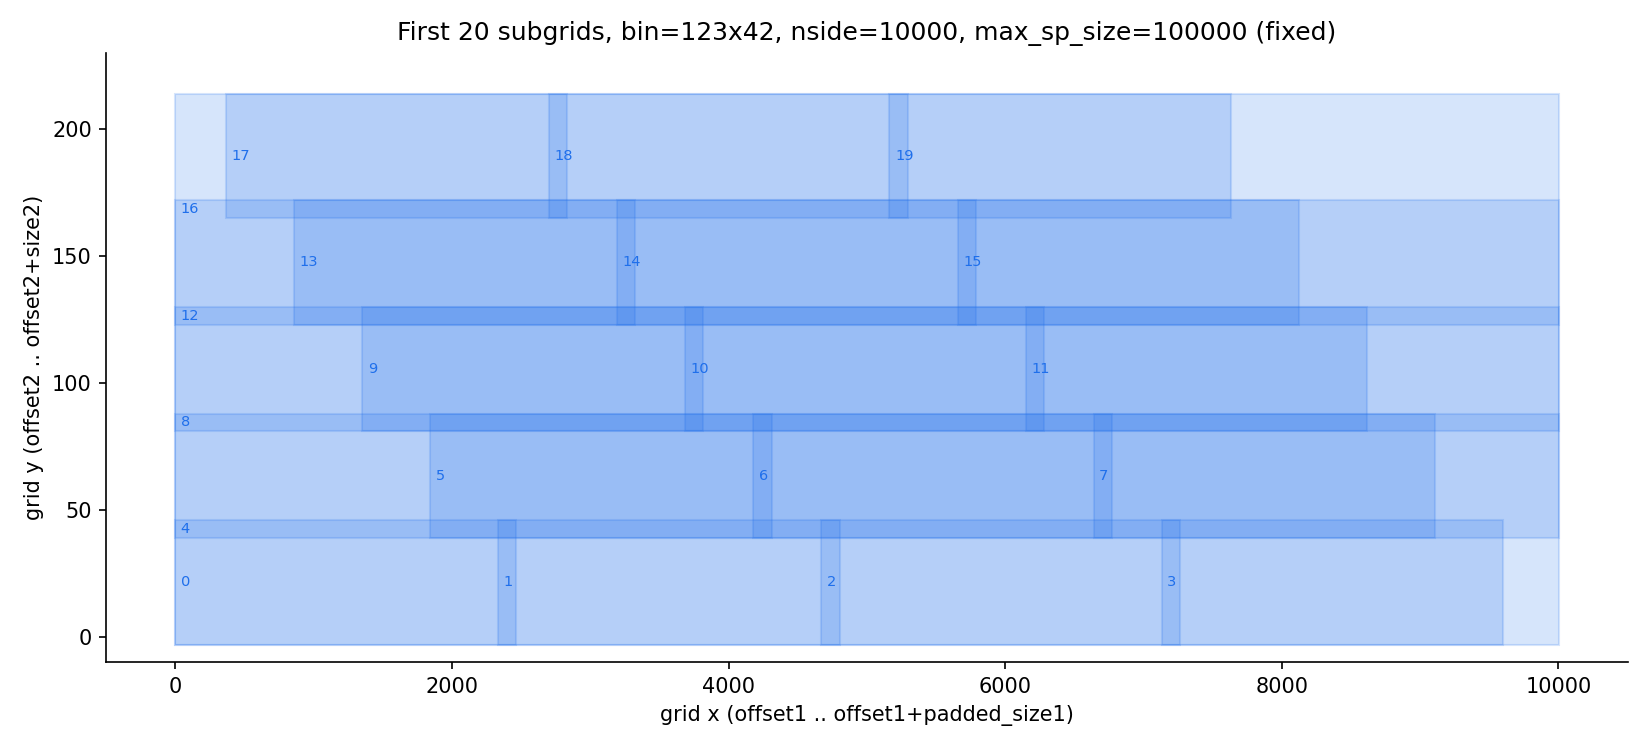
\includegraphics[width=\textwidth]{figures/bin_size/subgrid_overlap_first20.png}
%        \caption{First 20 subgrids}
%        \label{fig:subgrid_overlap}
%    \end{subfigure}
%    \hfill
%    \begin{subfigure}[b]{0.48\textwidth}
%        \centering
%        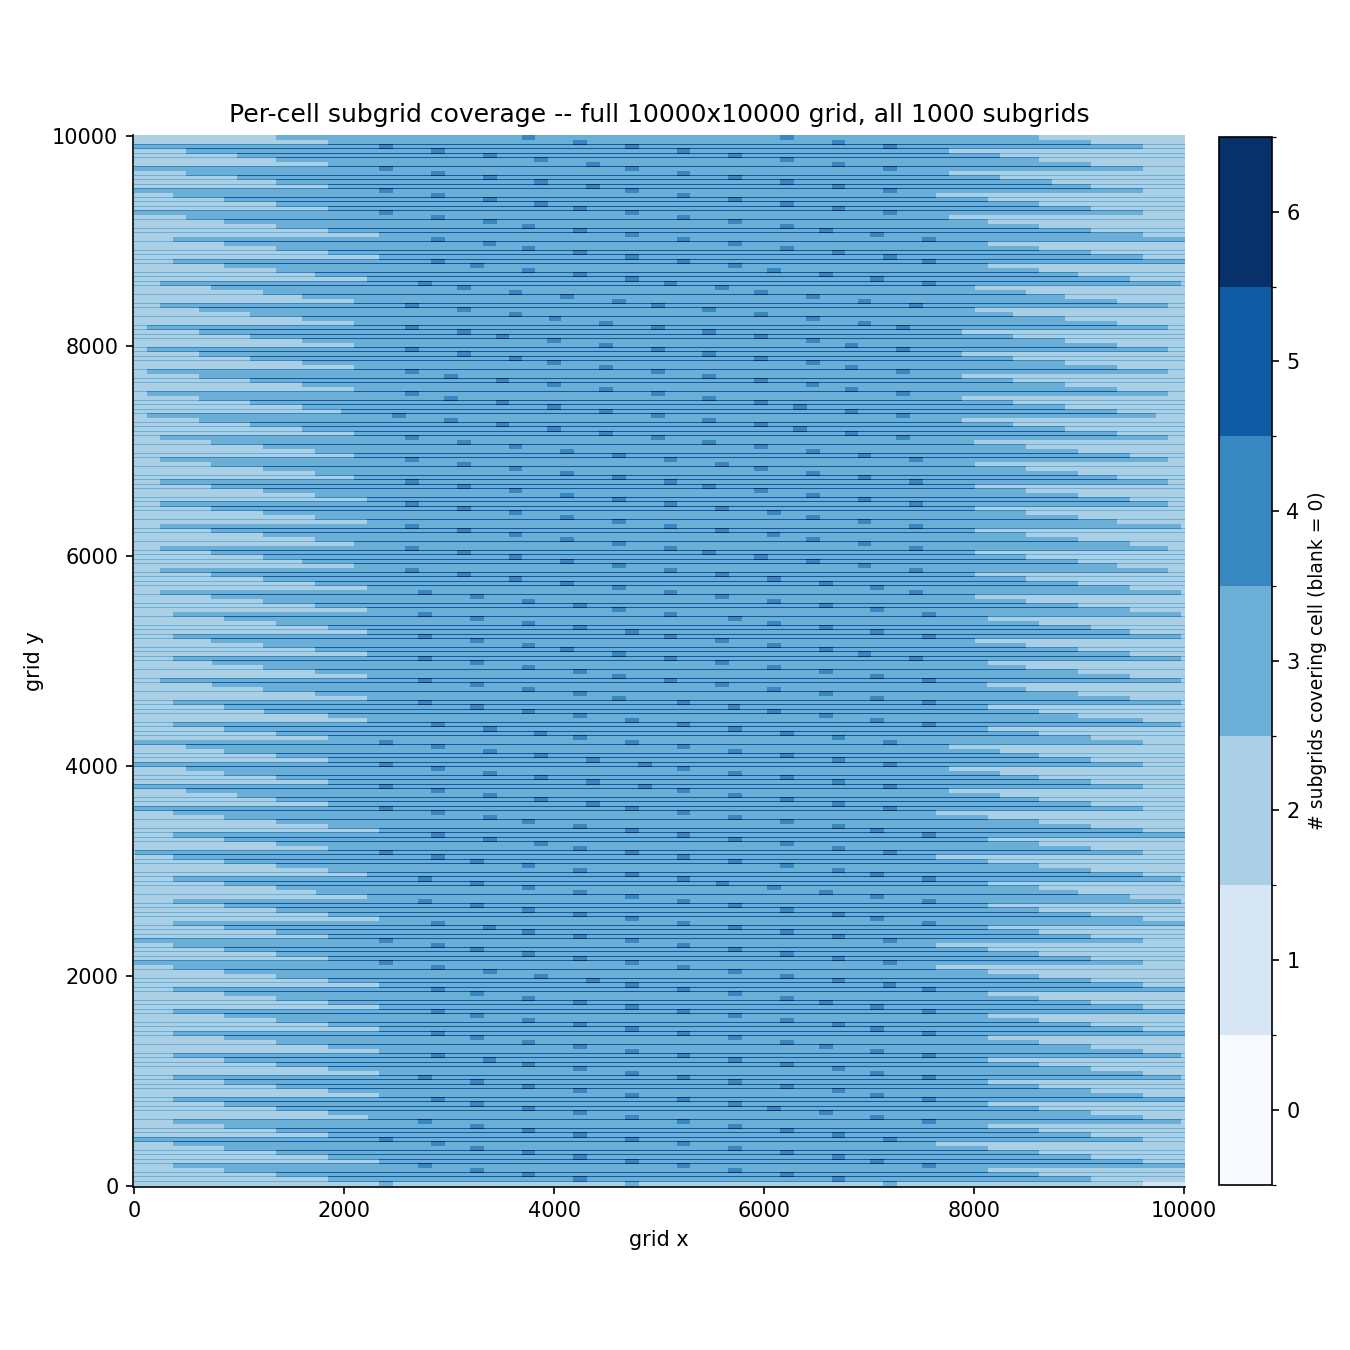
\includegraphics[width=\textwidth]{figures/bin_size/subgrid_coverage_heatmap.png}
%        \caption{Per-cell subgrid coverage, full grid}
%        \label{fig:subgrid_coverage}
%    \end{subfigure}
%    \caption{Overlap between subgrids during accumulation, at bin size $123\times42$, $n_{\text{side}}=10000$, $S_{\max}=10^5$ (fixed). (a) The bounding boxes of the first 20 subgrids, illustrating how neighbouring subgrids overlap along both axes. (b) The number of subgrids writing to each cell of the full $10000\times10000$ grid, across all 1000 subgrids.}
%    \label{fig:subgrid_overlap_coverage}
%\end{figure}
%
%\begin{table}[h]
%    \centering
%    \begin{tabular}{|l|l|}
%        \hline
%        \textbf{Bin size} & \textbf{Branch misses (K)} \\
%        \hline
%        1   & 1627.1  \\
%        \hline
%        2   & 1883.5  \\
%        \hline
%        4   & 1998.5  \\
%        \hline
%        8   & 2779.3  \\
%        \hline
%        16  & 3673.6  \\
%        \hline
%        20  & 3126.3  \\
%        \hline
%        24  & 3191.0  \\
%        \hline
%        28  & 3254.3  \\
%        \hline
%        30  & 3212.6  \\
%        \hline
%        32  & 4314.4  \\
%        \hline
%        64  & 6176.8  \\
%        \hline
%        128 & 8690.5  \\
%        \hline
%        256 & 12832.9 \\
%        \hline
%    \end{tabular}
%    \caption{Accumulation-step (\texttt{add\_wrapped\_subgrid}) branch-miss counts (sampled via \texttt{perf record}, averaged over 5 runs) as a function of bin size, for $M=4\times10^8$ nonuniform points under a uniform distribution, at $T=20$ threads, on an AMD Genoa processor.}
%    \label{tab:accum_branch_binsize}
%\end{table}

\section{Combined Heuristic}

\section{Summary}

% TODO: summarize findings and transition to conclusion
